% Options for packages loaded elsewhere
\PassOptionsToPackage{unicode}{hyperref}
\PassOptionsToPackage{hyphens}{url}
\PassOptionsToPackage{dvipsnames,svgnames,x11names}{xcolor}
%
\documentclass[
  a4paper,
  DIV=11,
  numbers=noendperiod]{scrartcl}

\usepackage{amsmath,amssymb}
\usepackage{iftex}
\ifPDFTeX
  \usepackage[T1]{fontenc}
  \usepackage[utf8]{inputenc}
  \usepackage{textcomp} % provide euro and other symbols
\else % if luatex or xetex
  \usepackage{unicode-math}
  \defaultfontfeatures{Scale=MatchLowercase}
  \defaultfontfeatures[\rmfamily]{Ligatures=TeX,Scale=1}
\fi
\usepackage{lmodern}
\ifPDFTeX\else  
    % xetex/luatex font selection
\fi
% Use upquote if available, for straight quotes in verbatim environments
\IfFileExists{upquote.sty}{\usepackage{upquote}}{}
\IfFileExists{microtype.sty}{% use microtype if available
  \usepackage[]{microtype}
  \UseMicrotypeSet[protrusion]{basicmath} % disable protrusion for tt fonts
}{}
\makeatletter
\@ifundefined{KOMAClassName}{% if non-KOMA class
  \IfFileExists{parskip.sty}{%
    \usepackage{parskip}
  }{% else
    \setlength{\parindent}{0pt}
    \setlength{\parskip}{6pt plus 2pt minus 1pt}}
}{% if KOMA class
  \KOMAoptions{parskip=half}}
\makeatother
\usepackage{xcolor}
\usepackage[margin=1in]{geometry}
\setlength{\emergencystretch}{3em} % prevent overfull lines
\setcounter{secnumdepth}{5}
% Make \paragraph and \subparagraph free-standing
\makeatletter
\ifx\paragraph\undefined\else
  \let\oldparagraph\paragraph
  \renewcommand{\paragraph}{
    \@ifstar
      \xxxParagraphStar
      \xxxParagraphNoStar
  }
  \newcommand{\xxxParagraphStar}[1]{\oldparagraph*{#1}\mbox{}}
  \newcommand{\xxxParagraphNoStar}[1]{\oldparagraph{#1}\mbox{}}
\fi
\ifx\subparagraph\undefined\else
  \let\oldsubparagraph\subparagraph
  \renewcommand{\subparagraph}{
    \@ifstar
      \xxxSubParagraphStar
      \xxxSubParagraphNoStar
  }
  \newcommand{\xxxSubParagraphStar}[1]{\oldsubparagraph*{#1}\mbox{}}
  \newcommand{\xxxSubParagraphNoStar}[1]{\oldsubparagraph{#1}\mbox{}}
\fi
\makeatother


\providecommand{\tightlist}{%
  \setlength{\itemsep}{0pt}\setlength{\parskip}{0pt}}\usepackage{longtable,booktabs,array}
\usepackage{calc} % for calculating minipage widths
% Correct order of tables after \paragraph or \subparagraph
\usepackage{etoolbox}
\makeatletter
\patchcmd\longtable{\par}{\if@noskipsec\mbox{}\fi\par}{}{}
\makeatother
% Allow footnotes in longtable head/foot
\IfFileExists{footnotehyper.sty}{\usepackage{footnotehyper}}{\usepackage{footnote}}
\makesavenoteenv{longtable}
\usepackage{graphicx}
\makeatletter
\newsavebox\pandoc@box
\newcommand*\pandocbounded[1]{% scales image to fit in text height/width
  \sbox\pandoc@box{#1}%
  \Gscale@div\@tempa{\textheight}{\dimexpr\ht\pandoc@box+\dp\pandoc@box\relax}%
  \Gscale@div\@tempb{\linewidth}{\wd\pandoc@box}%
  \ifdim\@tempb\p@<\@tempa\p@\let\@tempa\@tempb\fi% select the smaller of both
  \ifdim\@tempa\p@<\p@\scalebox{\@tempa}{\usebox\pandoc@box}%
  \else\usebox{\pandoc@box}%
  \fi%
}
% Set default figure placement to htbp
\def\fps@figure{htbp}
\makeatother

\KOMAoption{captions}{tableheading}
\makeatletter
\@ifpackageloaded{caption}{}{\usepackage{caption}}
\AtBeginDocument{%
\ifdefined\contentsname
  \renewcommand*\contentsname{Table of contents}
\else
  \newcommand\contentsname{Table of contents}
\fi
\ifdefined\listfigurename
  \renewcommand*\listfigurename{List of Figures}
\else
  \newcommand\listfigurename{List of Figures}
\fi
\ifdefined\listtablename
  \renewcommand*\listtablename{List of Tables}
\else
  \newcommand\listtablename{List of Tables}
\fi
\ifdefined\figurename
  \renewcommand*\figurename{Figure}
\else
  \newcommand\figurename{Figure}
\fi
\ifdefined\tablename
  \renewcommand*\tablename{Table}
\else
  \newcommand\tablename{Table}
\fi
}
\@ifpackageloaded{float}{}{\usepackage{float}}
\floatstyle{ruled}
\@ifundefined{c@chapter}{\newfloat{codelisting}{h}{lop}}{\newfloat{codelisting}{h}{lop}[chapter]}
\floatname{codelisting}{Listing}
\newcommand*\listoflistings{\listof{codelisting}{List of Listings}}
\makeatother
\makeatletter
\makeatother
\makeatletter
\@ifpackageloaded{caption}{}{\usepackage{caption}}
\@ifpackageloaded{subcaption}{}{\usepackage{subcaption}}
\makeatother

\usepackage{bookmark}

\IfFileExists{xurl.sty}{\usepackage{xurl}}{} % add URL line breaks if available
\urlstyle{same} % disable monospaced font for URLs
\hypersetup{
  pdftitle={Forcasting Daily Online Retails Sales using SARIMAX model},
  pdfkeywords={Metaphysics, String Theory},
  colorlinks=true,
  linkcolor={blue},
  filecolor={Maroon},
  citecolor={Blue},
  urlcolor={Blue},
  pdfcreator={LaTeX via pandoc}}


\title{Forcasting Daily Online Retails Sales using SARIMAX model}
\author{}
\date{2025-02-04}

\begin{document}
\maketitle

\renewcommand*\contentsname{Table of Contents}
{
\hypersetup{linkcolor=}
\setcounter{tocdepth}{3}
\tableofcontents
}

\section{Main Objective of the
Analysis}\label{main-objective-of-the-analysis}

The main objective of this analysis is to forecast future sales of
retail products based on historical sales data. The time series
forecasting model selected is a SARIMA (Seasonal AutoRegressive
Integrated Moving Average) model, which is well-suited for time series
data that exhibits both trend and seasonality, such as retail sales
data. By using this model, the business can gain valuable insights into
future sales, enabling better inventory management, demand planning, and
resource allocation. The analysis aims to help stakeholders, such as
supply chain managers, inventory planners, and marketing teams, make
informed decisions based on forecasted sales trends.

\section{Brief Description of the
Dataset}\label{brief-description-of-the-dataset}

The dataset chosen for this analysis is the Online Retail dataset from
the UCI Machine Learning Repository. The dataset contains transactional
data for a UK-based retail company, detailing purchases made by
customers between 2010 and 2011. The key attributes in the dataset
include:

\begin{itemize}
\tightlist
\item
  InvoiceNo: Unique identifier for each invoice.
\item
  StockCode: Product code for each item purchased.
\item
  Description: Product description.
\item
  Quantity: Number of units purchased.
\item
  InvoiceDate: Date and time when the invoice was generated.
\item
  UnitPrice: Price per unit of the product.
\item
  CustomerID: Unique identifier for customers.
\item
  Country: Country of the customer.
\end{itemize}

The primary objective of this analysis is to forecast the total sales
(Quantity * UnitPrice) for the company over a specified future period.
This forecast will aid the company in predicting demand and adjusting
its strategies for inventory and marketing.

\section{Data Exploration and Feature
Engineering}\label{data-exploration-and-feature-engineering}

\subsection{Data Exploration}\label{data-exploration}

The data exploration process involved inspecting the dataset for any
obvious issues or inconsistencies

There were no missing values or ouliers. So we proceed with the analysis

\subsection{Feature Engineering}\label{feature-engineering}

\begin{itemize}
\item
  The \texttt{InvoiceDate} column was parsed into datetime format to
  facilitate time series analysis.
\item
  The time series data was aggregated on a daily basis to calculate
  total sales for each day, considering the product of \texttt{Quantity}
  and \texttt{UnitPrice} and \texttt{Sales} column was created.
\end{itemize}

\section{Data Anlaysis}\label{data-anlaysis}

\begin{figure}[H]

{\centering \pandocbounded{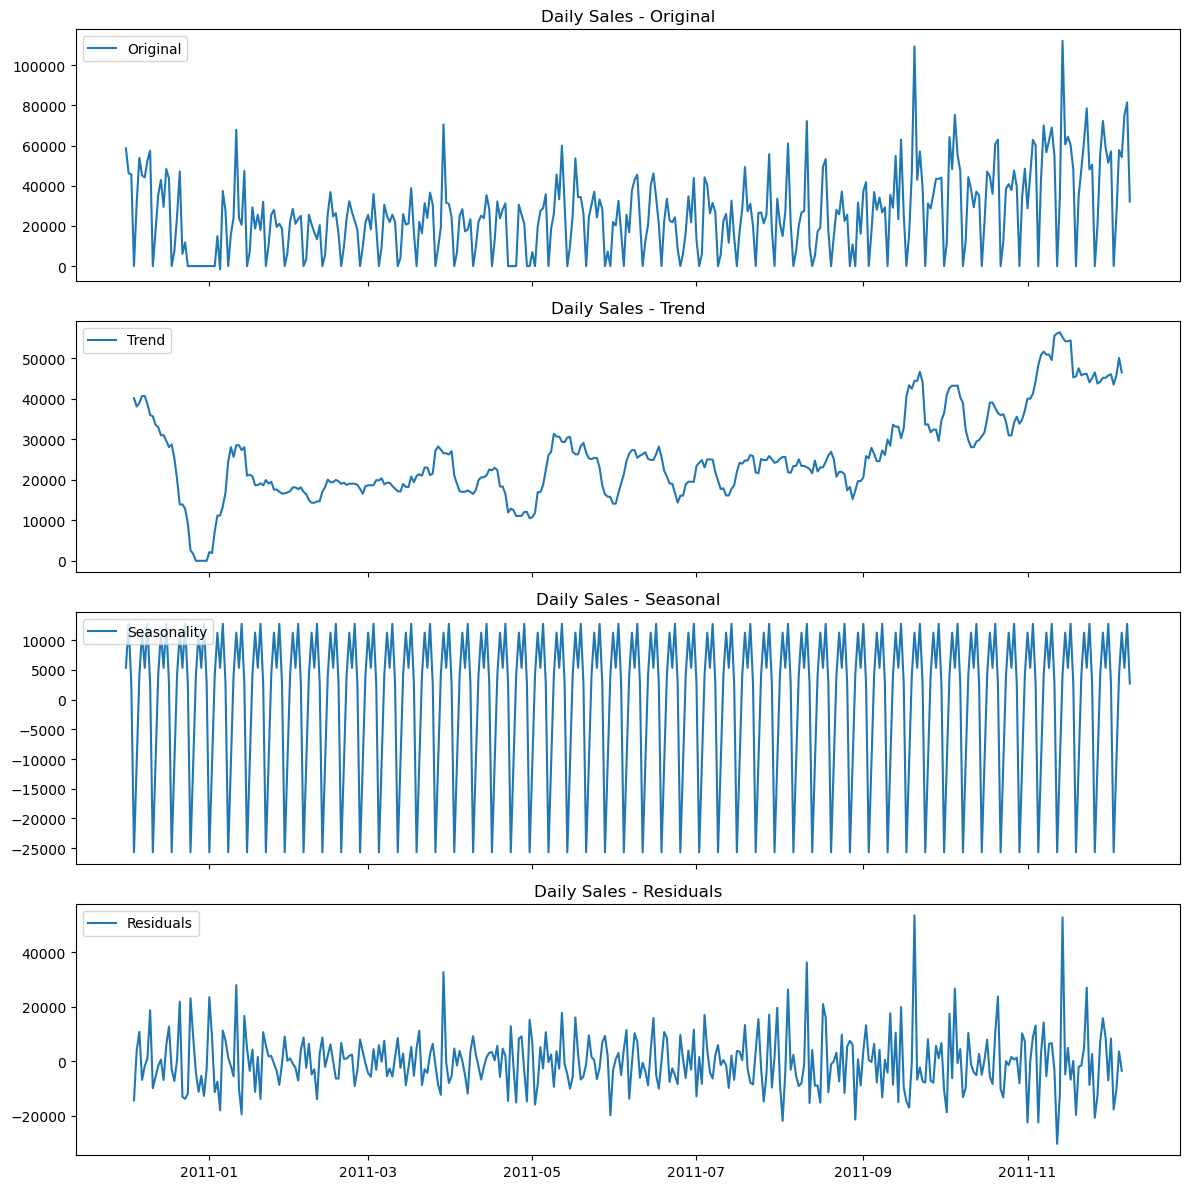
\includegraphics[keepaspectratio]{report_files/fig_1.png}}

}

\caption{Series, Trend, Seasonality, Residuals Diagram}

\end{figure}%

Figure 1 shows the decomposition of the components of the Time Series.
We can observer a slight trend and a clear weekly seasonl pattern

\begin{figure}[H]

{\centering \pandocbounded{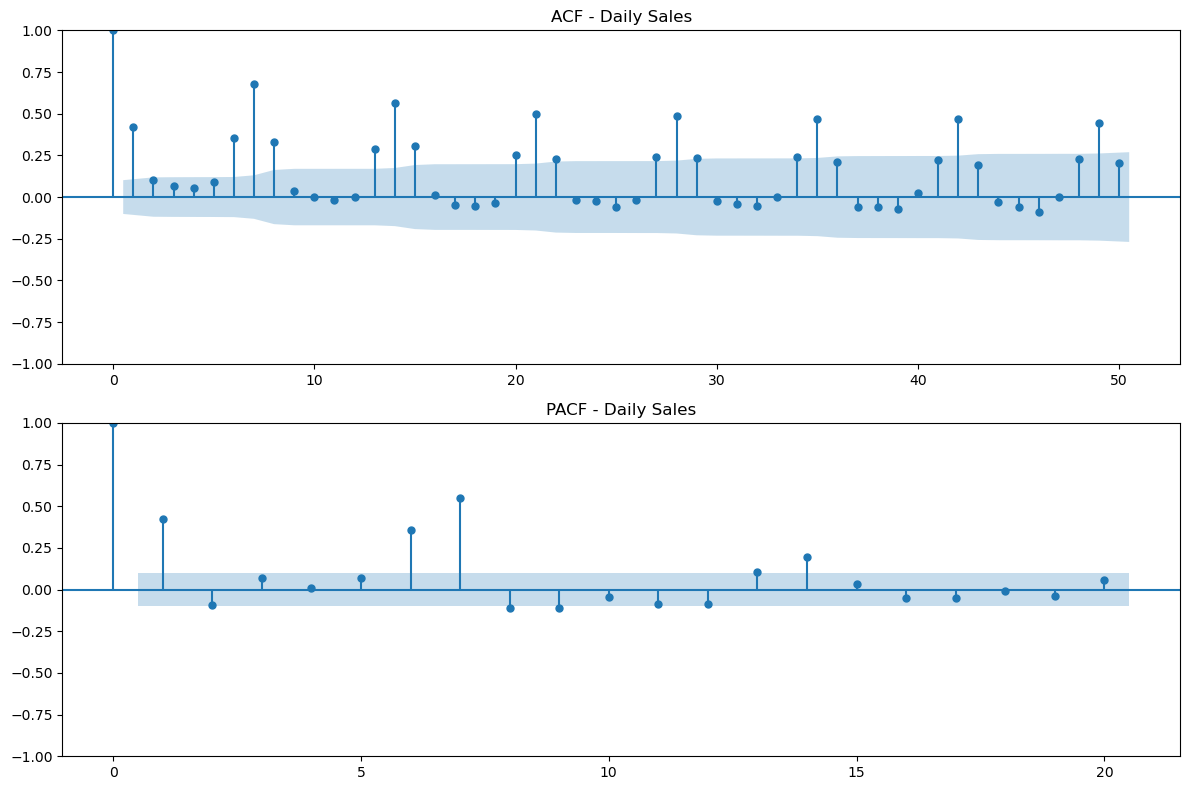
\includegraphics[keepaspectratio]{report_files/fig_2.png}}

}

\caption{ACF and PACF plots}

\end{figure}%

Figure 2 show the ACF and PACF plots. Here also we can clearly observe
that there is a weskly seasnality, as a result of seasonal lags been
significant.

\section{Methodology}\label{methodology}

The forecasting model for the daily sales data was built using two
distinct approaches: SARIMAX and Stepwise ARIMA. Both models were aimed
at capturing the temporal dependencies and seasonality inherent in the
data to make accurate predictions. The steps followed for each method
are outlined below:

\begin{enumerate}
\def\labelenumi{\arabic{enumi}.}
\tightlist
\item
  \textbf{SARIMAX Model:}

  \begin{itemize}
  \tightlist
  \item
    \textbf{Model Definition:} A SARIMAX model was specified with the
    following parameters:

    \begin{itemize}
    \tightlist
    \item
      \textbf{AR(1):} One autoregressive term to capture the dependence
      of the current sales on the previous day's sales.
    \item
      \textbf{MA(1) Seasonal Component:} A seasonal moving average term
      at lag 7 to account for weekly seasonal patterns in the sales
      data.
    \item
      \textbf{Trend:} A constant trend was added to the model to capture
      any potential upward or downward trends over time.
    \end{itemize}
  \item
    \textbf{Model Fitting:} The SARIMAX model was fit using the
    \texttt{sm.tsa.statespace.SARIMAX} function from the
    \texttt{statsmodels} library. The model was trained on the
    historical data, and the optimal parameters were estimated using
    maximum likelihood estimation.
  \end{itemize}
\item
  \textbf{Stepwise ARIMA Model:}

  \begin{itemize}
  \tightlist
  \item
    \textbf{Model Definition:} The stepwise ARIMA model was chosen using
    the \texttt{auto\_arima} function from the \texttt{pmdarima}
    library. This function automates the process of selecting the best
    ARIMA model by evaluating different combinations of parameters:

    \begin{itemize}
    \tightlist
    \item
      \textbf{AR(p), MA(q):} A range of values from 1 to 3 were tested
      for both AR and MA components.
    \item
      \textbf{Seasonal Parameters (P, Q):} The model was defined to have
      a seasonal component with a period of 7 (weekly seasonality), with
      seasonal MA terms considered at lags 7 and 14.
    \item
      \textbf{Differencing (d, D):} The model applied a non-seasonal
      differencing of order 0 and seasonal differencing of order 1 to
      make the series stationary.
    \end{itemize}
  \item
    \textbf{Model Fitting:} The \texttt{auto\_arima} function iterated
    through all possible combinations of parameters and selected the
    best model based on the AIC score. This resulted in the optimal
    configuration of ARIMA(1,0,1)(0,1,2){[}7{]}.
  \end{itemize}
\item
  \textbf{Model Evaluation:}

  \begin{itemize}
  \tightlist
  \item
    Both models were evaluated based on their \textbf{AIC (Akaike
    Information Criterion)} and \textbf{BIC (Bayesian Information
    Criterion)} values, with lower values indicating better model fit.
    Additionally, the \textbf{Ljung-Box test} was applied to the
    residuals of both models to check for autocorrelation and ensure
    that the models had adequately captured the temporal dependencies in
    the data.
  \end{itemize}
\end{enumerate}

By following these steps, the two models were built and evaluated to
identify the best approach for forecasting daily sales. The SARIMAX
model was initially fit to the data, but the stepwise ARIMA model, with
its automatic parameter selection, provided a more accurate and
parsimonious model.

\section{Results}\label{results}

\begin{enumerate}
\def\labelenumi{\arabic{enumi}.}
\tightlist
\item
  \textbf{SARIMAX Model:}
\end{enumerate}

\begin{verbatim}
Dep. Variable:  Sale    No. Observations:   374
Model:  SARIMAX(1, 0, 0)x(0, 1, [1], 7) Log Likelihood  -3994.175
Date:   Tue, 04 Feb 2025    AIC 7996.351
Time:   14:20:07    BIC 8011.972
Sample: 12-01-2010  HQIC    8002.557
- 12-09-2011        
Covariance Type:    opg     
coef    std err z   P>|z|   [0.025  0.975]
intercept   119.1026    237.682 0.501   0.616   -346.745    584.951
ar.L1   0.2701  0.069   3.899   0.000   0.134   0.406
ma.S.L7 -0.7873 0.048   -16.521 0.000   -0.881  -0.694
sigma2  2.215e+08   0.002   1.42e+11    0.000   2.22e+08    2.22e+08
Ljung-Box (L1) (Q): 0.74    Jarque-Bera (JB):   328.25
Prob(Q):    0.39    Prob(JB):   0.00
Heteroskedasticity (H): 1.80    Skew:   1.07
Prob(H) (two-sided):    0.00    Kurtosis:   7.11
\end{verbatim}

The SARIMAX model, with one autoregressive (AR) term, one seasonal
moving average term (MA) at lag 7, and a constant trend, produced an AIC
of 7996.351 and a BIC of 8011.972. The Ljung-Box test revealed no
significant autocorrelation in the residuals (p-value = 0.39),
indicating that the model effectively captured the patterns in the data.
Despite the absence of residual autocorrelation, the higher AIC and BIC
values compared to the stepwise ARIMA model suggest that the model's
performance can be improved

\begin{enumerate}
\def\labelenumi{\arabic{enumi}.}
\setcounter{enumi}{1}
\tightlist
\item
  \textbf{Stepwise ARIMA Model:}
\end{enumerate}

\begin{verbatim}
Dep. Variable:  y   No. Observations:   374
Model:  SARIMAX(1, 0, 1)x(0, 1, [1, 2], 7)  Log Likelihood  -3984.125
Date:   Tue, 04 Feb 2025    AIC 7980.251
Time:   16:11:56    BIC 8003.683
Sample: 12-01-2010  HQIC    7989.561
- 12-09-2011        
Covariance Type:    opg     
coef    std err z   P>|z|   [0.025  0.975]
intercept   56.6926 72.460  0.782   0.434   -85.327 198.713
ar.L1   0.8607  0.113   7.598   0.000   0.639   1.083
ma.L1   -0.6928 0.152   -4.557  0.000   -0.991  -0.395
ma.S.L7 -0.7252 0.076   -9.496  0.000   -0.875  -0.576
ma.S.L14    -0.1233 0.074   -1.657  0.098   -0.269  0.023
sigma2  2.213e+08   8.55e-05    2.59e+12    0.000   2.21e+08    2.21e+08
Ljung-Box (L1) (Q): 0.08    Jarque-Bera (JB):   379.84
Prob(Q):    0.77    Prob(JB):   0.00
Heteroskedasticity (H): 2.04    Skew:   1.17
Prob(H) (two-sided):    0.00    Kurtosis:   7.40
\end{verbatim}

The stepwise ARIMA model identified a combination of one AR term, one MA
term, and two seasonal MA terms (at lags 7 and 14) as the optimal
configuration. This model achieved a lower AIC of 7980.251 and a BIC of
8003.683, signifying a better fit to the data compared to the SARIMAX
model. The Ljung-Box Q-test (p-value = 0.77) confirmed that the
residuals were white noise, further supporting the adequacy of the
model. The inclusion of the seasonal MA terms (lag 7 and lag 14) helped
capture additional seasonality that the SARIMAX model could not

\section{Conclusion}\label{conclusion}

In conclusion, the stepwise ARIMA model outperforms the SARIMAX model
(1, 0, 1)(0, 1, 2){[}7{]} based on the AIC, BIC, and residual
diagnostics, making it the preferred model for forecasting future sales.

\section{Key Findings and Insights}\label{key-findings-and-insights}

\begin{itemize}
\item
  Seasonality: The dataset showed strong weekly seasonality, which was
  effectively captured by the SARIMA model. This suggests that certain
  days of the week consistently perform better in terms of sales.
\item
  Trend: The sales data exhibited a positive trend, indicating growing
  demand over time.
\item
  Forecasting Future Sales: The SARIMA model provided reliable forecasts
  of future sales, with the ability to estimate the impact of seasonal
  patterns. These findings provide the business with actionable insights
  for resource planning, inventory management, and marketing strategies.
\end{itemize}

\section{Suggestions for Next Steps}\label{suggestions-for-next-steps}

Incorporating Deep Learning: Deep learning models (e.g., LSTM or RNN)
could provide better result




\end{document}
